
% ==================================================
%	Auswertung
% ==================================================

\section{Auswertung}
\label{sec:auswertung}

\subsection{Vertikalkomponente des Erdmagnetfelds}
\label{sub:vertikalkomponente_des_erdmagnetfelds}

Der Einfluss der Vertikalkomponente des Erdmagnetfelds wird dadurch
kompensiert, dass eine Helmholtzspule entsprechend gedreht und der Strom $I$ der
Spule so eingestellt wird, dass das induzierte Magnetfeld $B$ der
Vertikalkomponente entgegenwirkt. Das Magnetfeld kann nun mit Hilfe des
Biot-Savart-Gesetzes
\begin{equation}
  B = \upmu_0 \frac{8}{\sqrt{125}} \frac{I N}{r}
  \label{eq:biot}
\end{equation}
bestimmt werden.
Hierbei ist $\upmu_0$ die Vakuumpermeabilität, $r$ der Radius der Spule und $N$
die Windungszahl der Spule. Mit Hilfe der Kenndaten aus
Tabelle~\ref{tab:kenndaten_spulen} ergibt sich die Vertikalkomponente zu
\begin{equation}
  B_\text{vertikal} = \SI{36.2}{\micro\tesla}
\end{equation}

\begin{table}[htpb]
  \centering
  \begin{tabular}{lccc}
    \midrule
    \midrule
    Spule & $r$ in \si{\centi\meter} & $N$ & $I/U$ in \si{\ampere} \\
    \midrule
    Vertikal   & 11.735           & \phantom{0}20 & 0.1 \\
    Horizontal & 15.790           & 154           & 0.3 \\
    Sweep      & 16.39\phantom{0} & \phantom{0}11 & 0.1 \\
    \midrule
    \midrule
  \end{tabular}
  \caption{Kenndaten der verwandten Helmholtzspulen. Hierbei bezeichnet $r$ den
    Spulenradius, $N$ die Windungszahl und $I/U$ den Strom pro Umdrehung des
    Potentiometers.}
\label{tab:kenndaten_spulen}
\end{table}

\subsection{Horizontalkomponente des Erdmagnetfelds}
\label{sub:horizontalkomponente_des_erdmagnetfelds}

Die in Teil 2 von Abschnitt~\ref{sub:durchfuehrung} aufgenommenen Werte
für die beiden Isotope befinden sich in Tabelle~\ref{tab:isotop}
Hierin sind die Umdrehungen der
Potentiometer der Sweep- und Horizontalfeldspule in Abhängigkeit der
RF-Frequenz dargestellt sowie die entsprechend~\eqref{eq:biot} und den Werten
aus Tabelle~\ref{tab:kenndaten_spulen} errechneten Magnetfeldstärken $B$, wobei
sich die Feldstärken der Spulen addieren. Die Wertepaare $\nu$ und $B$ werden
nun linear gefittet. Die Messwerte sowie die Fits für beide Istotope sind in
Abbildung~\ref{fig:isotop} dargestellt.
Die durch den Fit erhaltenen Geradengleichungen lauten für das erste Isotop
\begin{equation}
  G_1(\nu) = \SI[parse-numbers = false]{(0.1446 \pm 0.0014)}{\micro\tesla\per\kilo\hertz}\, \cdot \,\nu\, + \SI[parse-numbers = false]{(19.7 \pm 0.8)}{\micro\tesla}
  \label{eq:gerade_1}
\end{equation}
und für das zweite Isotop
\begin{equation}
  G_2(\nu) = \SI[parse-numbers = false]{(0.2118 \pm 0.0024)}{\micro\tesla\per\kilo\hertz}\, \cdot \,\nu\, + \SI[parse-numbers = false]{(21.2 \pm 1.5)}{\micro\tesla}~.
  \label{eq:gerade_2}
\end{equation}
Die Horizontalkomponente des Erdmagnetfelds ist nun das Magnetfeld bei $\nu =
0$ und somit der $y$-Abschnitt der Geraden. Somit folgen die
Horizontalkomponenten
\begin{equation}
  B_1 = \SI[parse-numbers = false]{(19.7 \pm 0.8)}{\micro\tesla}\qquad \text{und} \qquad
  B_2 = \SI[parse-numbers = false]{(21.2 \pm 1.5)}{\micro\tesla}
\end{equation}
sowie deren Mittelwert
\begin{equation}
  B_\text{hor} = \SI[parse-numbers = false]{(20.4 \pm 0.8)}{\micro\tesla}~.
\end{equation}

\begin{table}[htpb]
  \centering
  \begin{tabular}{c|cc||c|cc||c}
      \midrule
      \midrule
      & \multicolumn{3}{c|}{Isotop 1} &
      \multicolumn{3}{c}{Isotop 2} \\
      \midrule
      $\nu$ in \si{\kilo\hertz} & $U_\text{sweep} $ & $U_\text{hor}$ & $B$ in
      \si{\milli\tesla} &
      $U_\text{sweep} $ & $U_\text{hor}$ & $B$ in
      \si{\milli\tesla} \\
      \midrule
      \phantom{0}100\phantom{.} & 5.54              & 0.00              & 0.033             & 6.73              & 0.00              & 0.041            \\
\phantom{0}204\phantom{.} & 5.92              & 0.05              & 0.049             & 8.31              & 0.05              & 0.063            \\
\phantom{0}296\phantom{.} & 3.54              & 0.16              & 0.063             & 7.03              & 0.16              & 0.085            \\
\phantom{0}400\phantom{.} & 2.14              & 0.25              & 0.079             & 6.78              & 0.25              & 0.107            \\
\phantom{0}502\phantom{.} & 3.23              & 0.28              & 0.093             & 9.19              & 0.28              & 0.129            \\
\phantom{0}607\phantom{.} & 1.77              & 0.36              & 0.105             & 8.94              & 0.36              & 0.149            \\
\phantom{0}699\phantom{.} & 0.81              & 0.44              & 0.121             & 9.08              & 0.44              & 0.171            \\
\phantom{0}804\phantom{.} & 2.91              & 0.45              & 0.136             & 5.92              & 0.60              & 0.194            \\
\phantom{0}901\phantom{.} & 5.31              & 0.45              & 0.150             & 6.60              & 0.66              & 0.213            \\
1003\phantom{.}   & 5.20              & 0.78              & 0.237             & 7.02              & 0.71              & 0.229            \\
      \midrule
      \midrule
    \end{tabular}
    \caption{Werte der Umdrehungen der Potentiometer für die Sweep- und
      Horizontalfeldspule $U_\text{sweep}$ bzw. $U_\text{hor}$
      in Abhängigkeit der RF-Frequenz $\nu$ für beide Isotope.
      Zudem sind die errechneten Magnetfeldstärken $B$ angegeben.}
    \label{tab:isotop}
\end{table}

\begin{figure}[htpb]
  \centering
  \includegraphics[scale=1.0]{bilder/isotop.pdf}
  \caption{Darstellung der Magnetfeldstärke $B$ in Abhängigkeit der
    RF-Frequenz sowie des linearen Fits.}
\label{fig:isotop}
\end{figure}

\clearpage
\subsection{Land\'{e}-Faktoren}
\label{sub:lande_faktoren_des_atoms}

Aus den Gleichungen~\eqref{eq:gerade_1} und~\eqref{eq:gerade_2} lassen sich mit
Hilfe der Gleichung~\eqref{eq:Bm}
die Land\'{e}-Faktoren der Hyperfeinaufspaltung der Isotope bestimmen.
Die Steigung $m$ der Geraden entspricht somit genau dem Ausdruck
\begin{equation}
  m = \frac{4\pi m_0}{e_0 g_F}~,
\end{equation}
wobei $m_0$ die Masse des Elektrons ist. Umstellen dieser Gleichung nach $g_F$
liefert schließlich die Land\'{e}-Faktoren
\begin{equation}
  g_{F,1} = \SI[parse-numbers = false]{0.494 \pm 0.005}{} \qquad \text{und} \qquad
  g_{F,2} = \SI[parse-numbers = false]{0.337 \pm 0.004}{}
\end{equation}
Zudem kann der Land\'{e}-Faktor $g_J$ der Elektronenhülle bestimmt werden,
welcher zur Berechnung der Kernspins im nächsten Abschnitt benötigt wird.
Dazu werden die Drehimpulse aus der Elektronenkonfiguration von Rubidium
\cite{NUK}
zu
\begin{equation}
  L = 0, \qquad S = \frac12, \qquad J = L + S = \frac12, \qquad
  F = I + J = I + \frac12
\end{equation}
abgelesen und der Land\'{e}-Faktor nach~\eqref{eq:g_J}
zu
\begin{equation}
  g_J = 2.0023
\end{equation}
bestimmt.

\subsection{Kernspin der Rb-Isotope}
\label{sub:kernspin_der_rb_isotope}

Mit Hilfe der Gleichung~\eqref{eq:g_F} und den Ergebnissen aus
Abschnitt~\ref{sub:lande_faktoren_des_atoms} kann nun der Kernspin $I$ der
jeweiligen Isotope bestimmt werden.
Das Umstellen der Formel~\eqref{eq:g_F} ergibt
\begin{equation}
  I = -1 + \frac{g_J}{4 g_F} +
  \sqrt{{\qty(1 - \frac{g_J}{4 g_F})}^2 - \qty(1 - \frac{g_J}{g_F})}~.
\end{equation}
Damit ergeben sich die Kernspins zu
\begin{equation}
  I_1 = \SI[parse-numbers = false]{1.760 \pm 0.021}{}, \qquad I_2 = \SI[parse-numbers = false]{2.757 \pm 0.035}{}
\end{equation}

\subsection{Isotopenverhältnis von \ce{^85Rb} und \ce{^87Rb}}
\label{sub:isotopenverhältnis_von_85_rb}

In Abbildung~\ref{fig:TEK} ist ein typisches Bild der Resonanzkurven am
Oszilloskop gezeigt. Die darin sichtbaren \enquote{Dips} lassen darauf
schließen, dass es sich um zwei verschiedene Isotope handelt.
Das Teilchenverhältnis der Isotope $N_i$ hängt dabei mit dem Verhältnis
der Transparenz $A_i$ entsprechend
\begin{equation}
  \frac{N_1}{N_2} = \frac{A_1}{A_2} = \frac{3.0}{1.5} = 2.0
\end{equation}
zusammen. Das Verhältnis wird hier bestimmt durch abzählen der Kästchen im
Oszilloskopenbild.

\begin{figure}[htpb]
  \centering
  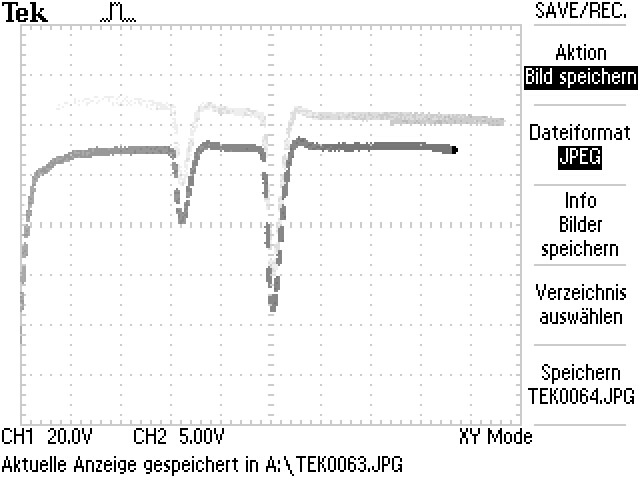
\includegraphics[scale=1.0]{bilder/TEK0066_rotated.JPG}
  \caption{Aufnahme der Resonanzkurven am Oszilloskop.}
\label{fig:TEK}
\end{figure}
